\documentclass{patmorin}
\usepackage{pat}
\usepackage{amsopn}
\listfiles

\DeclareMathOperator{\obs}{obs}
\newcommand{\x}{\mathsf{x}}
\newcommand{\y}{\mathsf{y}}

\title{\MakeUppercase{On Obstacle Numbers}}
\author{Vida Dujmovi\'c and Pat Morin}

\renewcommand{\note}[1]{}

\begin{document}
\begin{titlepage}
\maketitle

\begin{abstract}
\setlength{\baselineskip}{16.8pt}
The obstacle number is a new graph parameter introduced by Alpert, Koch,
and Laison (2010).  Mukkamala \etal\ (2012) show that there exist graphs
with $n$ vertices having obstacle number in $\Omega(n/\log n)$. In this
note, we up this lower bound to $\Omega(n/(\log\log n)^2)$.  Our proof
makes use of an upper bound of Mukkamala \etal\ on the number of graphs
having obstacle number at most $h$ in such a way that any subsequent
improvements to their upper bound will improve our lower bound.
\end{abstract}
\end{titlepage}


\section{Introduction}

\setlength{\baselineskip}{16.8pt}
The obstacle number is a new graph parameter introduced by Alpert, Koch,
and Laison \cite{alpert.koch.ea:obstacle}.  Let $G=(V,E)$ be a graph,
let $\varphi:V\to \R^2$ be a one-to-one mapping of the vertices of
$G$ onto $\R^2$ (hereafter called a \emph{drawing} of $G$), and let $S$
be a set of connected subsets of $\R^2$.  The pair $(\varphi,S)$ is an
\emph{obstacle representation} of $G$ when, for every pair of vertices
$u,w\in V$, the edge $uw$ is in $E$ if and only if the closed line
segment with endpoints $\varphi(u)$ and $\varphi(w)$ does not intersect
any \emph{obstacle} in $S$.\note{Changing open to closed handles obstacles
that sneak through vertices.}  An obstacle representation $(\varphi,S)$
is an \emph{$h$-obstacle} representation if $|S|=h$.  The \emph{obstacle
number} of a graph $G$, denoted by $\obs(G)$, is the minimum value of $h$
such that $G$ has an $h$-obstacle representation.\footnote{Note that
this definition of obstacle representation is more generous than that of Alpert, Koch, and Laison \cite{alpert.koch.ea:obstacle}, which requires that the obstacles be polygonal and that the
set of points determined by vertices of the obstacles and the image of $\varphi$ not contain 3 collinear points. Since the current
paper proves a lower-bound on the obstacle number, this lower bound
also applies to the original definition.}
\note{Obstacles that intersect each other is fine.}
\note{Changed $w(n)$ to $\obs(n)$}

Note that obstacle representations of planar graphs using few obstacles
often requires drawings of those graphs that are far from crossing free,
as the surprising example in \figref{fivebyfive} shows.  This example,
which shows a 1-obstacle representation of the $5\times 5$ grid graph,
$G_{5\times 5}$, that was given to us by Fabrizio Frati. In this figure,
the single obstacle is drawn as a shaded region. Since at least one
obstacle is clearly necessary to represent any graph other than a complete
graph, this proves that $\obs(G_{5\times 5}) = 1$.  (A similar drawing can
be used to show that the $a\times b$, grid graph has obstacle number 1,
for any integers $a,b>1$.)

\begin{figure}[hbpt]
  \begin{center}
    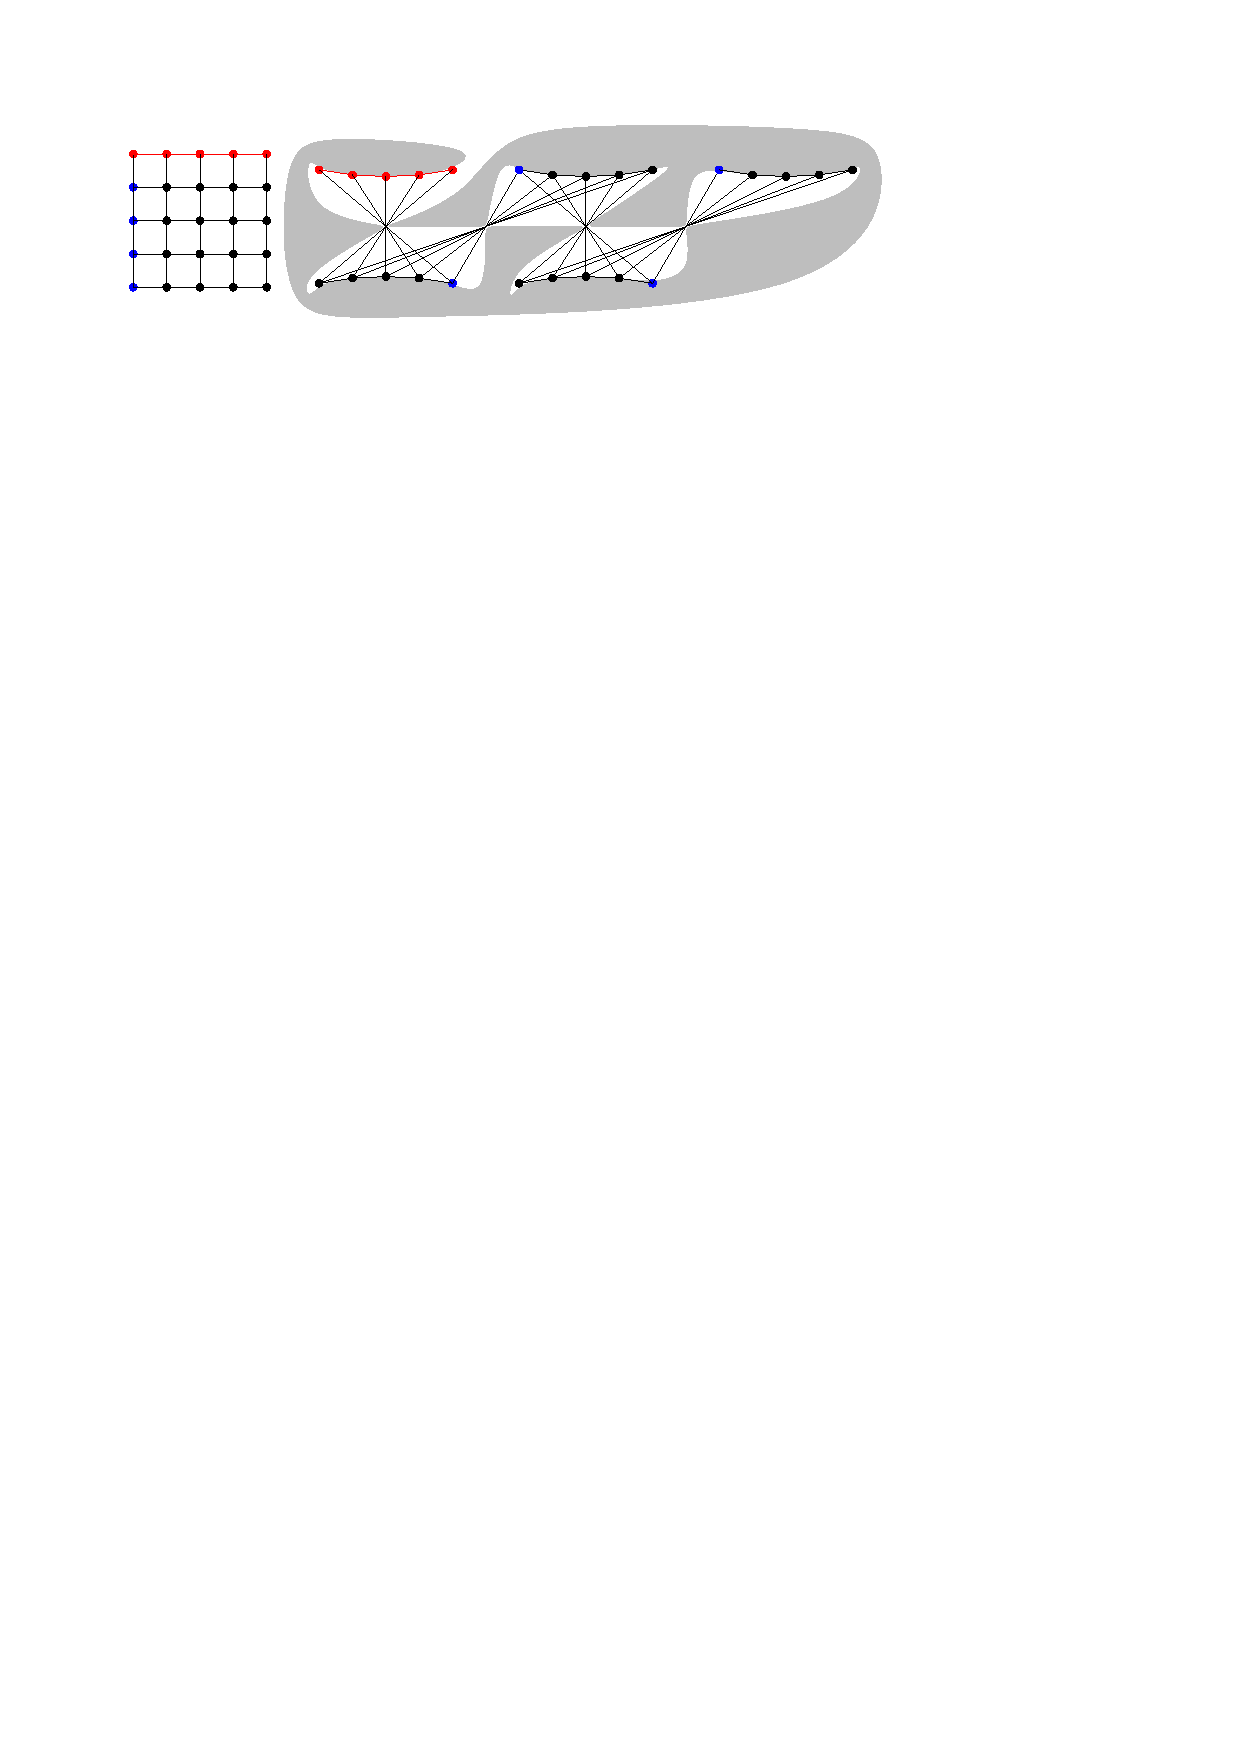
\includegraphics{fivebyfive}
  \end{center}  
  \caption{The $5\times 5$ grid graph has obstacle number 1.}
  \figlabel{fivebyfive}
\end{figure}

Since their introduction, obstacle numbers have generated significant
research interest 
\cite{%
   fulek.saeedi:convex,%
   johnson.sarioz:computing,%
   mukkamala.pach.ea:lower,%
   mukkamala.pach.ea:graphs,%
   pach.sarioz:small,%
   pach.sarioz:on,%
   sarioz:approximating%
}.
A fundamental---and far from answered---question about obstacle numbers
is that of determining the \emph{worst-case obstacle number},
\[
    \obs(n) = \max \{\obs(G) :\mbox{$G$ is a graph with $n$ vertices}\}
    \enspace ,
\] 
of a graph with $n$ vertices.

For a graph $G=(V,E)$, we call elements of $\binom{V}{2}\setminus E$
\emph{non-edges} of $G$.  The worst-case obstacle number $\obs(n)$ is
obviously upper-bounded by $\binom{n}{2}\in O(n^2)$ since, by mapping
the vertices of $G$ onto a point set in sufficiently general position,
one can place a small obstacle---even a single point---on the mid-point
of each non-edge of $G$.  No upper-bound on $\obs(n)$ that is asymptotically
better than $O(n^2)$ is known.

More is known about lower-bounds on $\obs(n)$.  Alpert, Koch, and Laison \cite{alpert.koch.ea:obstacle}
initially show that the worst-case obstacle number is
$\Omega\left(\sqrt{\log n/\log\log n}\right)$ and posed as an open problem the question
of determining if $\obs(n)\in\Omega(n)$.
%\footnote{Alpert \etal's lower-bound uses the Erd\H{o}s-Szekeres convex
%$n$-gon theorem and shows the existence of an $n$-vertex graph $G$
%with $\obs(G)\ge \sqrt{\log n/\log\log n}$.}
Mukkamala \etal\ \cite{mukkamala.pach.ea:graphs} showed that $\obs(n)\in
\Omega(n/\log^2 n)$ and Mukkamala \etal\ \cite{mukkamala.pach.ea:lower}
later increased this to $\obs(n)\in\Omega(n/\log n)$.  In the current paper,
we up the lower-bound again by proving the following theorem:
\begin{thm}\thmlabel{main}
  For every integer $n>0$, $\obs(n)\in\Omega(n/(\log\log n)^2)$, i.e., there
  exist graphs, $G$, with $n$ vertices and $\obs(G)\in\Omega(n/(\log\log
  n)^2)$.
\end{thm}

The proof of \thmref{main} makes use of an upper bound of Mukkamala \etal\
\cite[Theorem~1]{mukkamala.pach.ea:lower} on the number of graphs having
obstacle number at most $h$ in such a way that any subsequent improvements
on their upper bound will result in an improved lower bound on $\obs(n)$.

Although some aspects of our proof are a little technical, the main
idea is quite simple:  Mukkamala \etal\ \cite{mukkamala.pach.ea:lower}
show that, with probability at least $1-2^{-\Omega(n^2)}$, a random
graph on $n$ vertices has obstacle number at least $\Omega(n/(\log n)^2)$.
Our proof trades off a lower probability for a higher obstacle number.
When all is said and done, our proof shows that, with probability at least
$1-2^{-\Omega(n\log n)}$, a random graph on $n$ vertices has obstacle
number at least $n/(\log\log n)^2$.

\section{The Proof}

Our proof strategy is an application of the probabilistic method
\cite{alon.spencer:probabilistic}.  We consider the following
experiment: We fix an arbitrary drawing, $\varphi$, of a graph, $G$,
with vertex set $V=\{1,\ldots,n\}$ and then select each potential edge
$uw\in\binom{V}{2}$ to appear independently with probability $1/2$.
We show that the probability, $p$, that the drawing $\varphi$ allows
for an obstacle representation with few obstacles is extremely small.
We then show that the number, $N$, of combinatorially distinct drawing is
not too big.  Small and big in this case are defined so that $pN < 1$.
Therefore, by the union bound, there exists at least one graph, $G'$,
that has no drawing that allows for an obstacle representation with
few obstacles.  In other words, $\obs(G')$ is large.

\subsection{A Random Graph with a Fixed Drawing}

We make use of the following theorem, due to Mukkamala, Pach, and
P\'alv\"olgyi \cite[Theorem~1]{mukkamala.pach.ea:lower} about the number
of $n$ vertex graphs with obstacle number at most $h$:\note{We do need $h\ge 1$. With $h=0$, the upper bound is $O(1)$, but there are $n+1$ graphs with
\textbf{at most} $n$ vertices and obstacle number 0.}
\begin{thm}[Mukkamala, Pach, and P\'alv\"olgyi 2012]\thmlabel{pach-gang}
  For any $h\ge 1$, the number of graphs having $n$ vertices and
  obstacle number at most $h$ is at most $2^{O(hn\log^2 n)}$.
\end{thm}

Recall that an Erd\H{o}s-R\'enyi random graph $G_{n,\frac{1}{2}}$ is a
graph with $n$ vertices and each pair of vertices is chosen as an edge
or non-edge with equal probability and independently of every other pair
of vertices \cite{erdos.renyi:random}.  The following lemma shows that,
for random graphs, a fixed drawing is \emph{very} unlikely to yield
an obstacle representation with few obstacles.


\begin{lem}\lemlabel{fixed}
  Let $G=(V,E)$ be an Erd\H{o}s-R\'enyi random graph $G_{n,\frac{1}{2}}$,
  let $\varphi\from V\to \R^2$ be a one-to-one mapping that is
  independent of the choices of edges in $G$, and let $(\varphi, S)$ be
  an obstacle representation of $G$ using the minimum number of obstacles
  (subject to $\varphi$).  Then, for any constant $c>0$,
  \[
     \Pr\{|S| \in \Omega(n/(\log\log n)^2) \ge 1-e^{-cn\log n}  \enspace .
  \] 
  \note{Note to Pat: Come back and look at this $c$ again.}
\end{lem}

\begin{proof}
\note{We now specify that $k\in\omega(1)$ so that, later, $h\ge 1$.}
Let $P\subset\R^2$ denote the image of $\varphi$.  Fix some integer $k=k(n)\in\omega_n(1)$ to be
specified later and first consider some arbitrary subset $P'\subset P$
of $k$ points and let $G'=(V',E')$ be the subgraph of $G$ induced by
the set $V'=\{\varphi^{-1}(x):x\in P'\}$ of vertices that are mapped by
$\varphi$ to $P'$.  Applying \thmref{pach-gang} with $n=k$ and $h=\alpha
k/\log^2 k$, we obtain
\begin{equation}
     \Pr\{\obs(G') \le \alpha k/\log^2 k\} 
       \le \frac{2^{O(\alpha k^2)}}{2^{\binom{k}{2}}}
       = e^{-\beta k^2} \enspace , \eqlabel{g1}
\end{equation}
\note{Yes, $2^{\binom{k}{2}}$ is the number of possible Erd\H{o}s-R\'enyi random graphs (with a fixed vertex set). E-R graph is equivalent to random adjacency matrix.}%
for sufficiently small constants $\alpha,\beta > 0$.
Note that, if $\obs(G')\ge h$, then, in the obstacle representation
$(\varphi,S)$, there must be at least $h-1$ obstacles of $S$ that are
contained in the convex hull of $P'$.\note{This last statement is still
true for $h<1$ (because of the ``at least'').}

Without loss of generality assume that no two points in $P$ have the
same x-coordinate and denote the points in $P$ by $x_0,\ldots,x_{n-1}$
by increasing order of x-coordinate.  Let $m=\lfloor n/k\rfloor$ and
consider the point sets $P'_0,\ldots,P'_{m-1}$, where
\[ 
  P_i'=\{x_{ik},x_{ik+1},\ldots,x_{ik+k-1}\} \enspace .
\]  
That is, $P_0',\ldots,P_{m-1}'$ are determined by vertical slabs,
$s_0,\ldots,s_{m-1}$ that each contain $k$ points.  \Eqref{g1} shows
that, with probability at least $1-2^{-\Omega(k^2)}$, the obstacle number
of the subgraph that maps to $P'_i$ is $\Omega(k/\log^2 k)$.  If this
occurs, then $S$ has $\Omega(k/\log^2 k)$ obstacles that are completely
contained in the slab $s_i$.  These obstacles are therefore disjoint
from any other obstacles contained in any other slab $s_j$, $j\neq i$.

We are proving a lower bound on the number of obstacles, so we are
worried about the case where the number of slabs that do \emph{not}
contain at least $\alpha k/\log^2 k$ obstacles exceeds $m/e$.\footnote{Euler's constant $e=\lim_{n\rightarrow \infty} (1-1/n)^n$ is just a convenient
constant to use here.}
The number of slabs, $M$, not containing at least $\alpha k/\log^2 k$
obstacles is dominated by a binomial$(m,e^{-\beta k^2})$ random
variable.
\note{Vida asks if this is where we use E-R random graph property. Sort of---here we use that the edges within $P_i'$ are independent
of edges within $P_j'$ for $i\neq j$. (This is implicit in the claim
that there is an underlying binomial random variable.)}
Using Chernoff's bound on the tail of a binomial random
variable,\footnote{%
  Chernoff's Bound: For any binomial$(m,p)$ random variable, $B$,
  any $\delta>0$ and $\mu=mp$, 
  \[ \Pr\{B\ge (1+\delta)\mu\}
     \le \left(\frac{e^{\delta}}{(1+\delta)^{1+\delta}}\right)^{\mu} 
       \enspace . 
  \]}
we have that
\begin{align*}
  \Pr\{M \ge m/e\} & = \Pr\{M\ge (1+\delta)\mu\}
    & \text{(where $\mu=me^{-\beta k^2}$ and $\delta=e^{\beta k^2-1}-1$)} \\
    & \le \left(\frac{e^{\delta}}{(1+\delta)^{1+\delta}}\right)^{\mu} \\
    & \le \left(\frac{e^{e^{\beta k^2}}}{(e^{\beta k^2-1})^{e^{\beta k^2-1}}}\right)^{me^{-\beta k^2}}\\
    & = \left(\frac{e^{e^{\beta k^2}}}{e^{(\beta k^2-1)e^{\beta k^2-1}}}\right)^{me^{-\beta k^2}}\\
    & = \frac{e^{m}}{e^{m(\beta k^2-1)e^{\beta k^2-1}e^{-\beta k^2}}} \\
    & = \frac{e^{m}}{e^{m(\beta k^2-1)/e}} \\
    & = e^{-\Omega(mk^2)} \enspace .
\end{align*}
Taking $k=c'\log n$, for a sufficiently large constant, $c'$, and recalling that $m=\lfloor n/k\rfloor$, we obtain
the desired result.  In particular,
\[
    |S| \ge \Omega\left(\left(k/\log^2 k\right)\times m \right)
      = \Omega\left(n/(\log\log n)^2\right)
\]
with probability at least
\[
    1-e^{-\Omega(mk^2)} = 1-e^{-\Omega(c'n\log n)} \ge 1-e^{-cn\log n} \enspace . \qedhere
\]
\end{proof}

We have completed the first step in our application of the probabilistic
method.  \lemref{fixed} shows that the probability, $p$, that a
particular drawing of the random graph $G$ is able to yield an obstacle
representation with $o(n/(\log\log n)^2)$ obstacles is extremely small.
The remaining difficulty is establishing a sufficiently strong upper-bound
on $N$, the number of drawings of $G$. In actuality, the number of
drawings is uncountable.  However, we are interested in the number of
``combinatorially distinct'' drawings.  In particular, we would like
to partition the set of drawings into equivalence classes such that,
within each equivalence class, the minimum number of obstacles in an
obstacle representation remains the same.

Classifying drawings (i.e., labelled sets or sequences of $n$
points) into combinatorially distinct equivalence classes has
been considered previously. Several definitions of equivalence
exist, including oriented matroid (a.k.a., chirotope) equivalence
\cite{bland.vergnas:orientability,folkman.lawrence:oriented}, semispace
equivalence \cite{goodman.pollack:semispaces}, order equivalence
\cite{goodman.pollack:multidimensional}, and combinatorial equivalence
\cite{goodman:on,goodman.pollack:semispaces}.  For the latter two
definitions of equivalence, the number of distinct (equivalence classes
of) point sequences is $e^{O(n\log n)}$ \cite{goodman.pollack:upper}.

%Definitions include equivalence classes of point
%sets with the same \emph{order type} \cite{goodman.pollack:upper}, in which the orientation
%of every triple of points is preserved and equivalence classes of point
%sets with the same \emph{combinatorial-type}, in which a labelled point
%set is identified with the periodic sequence of permutations obtained
%by orthogonally projecting the points onto a line that rotates around
%a fixed point \cite{goodman.pollack:}.  Under both definitions, the number of distinct
%(equivalence classes of) point sets is $e^{O(n\log n)}$

Unfortunately, neither order types nor combinatorial-types are
sufficient for answering questions about obstacle representations.\note{Those other types don't have upper bounds on their numbers, so even if they're strong enough, we'd still have to prove upper bounds. It didn't look like those other types would work either but, to be honest, I didn't untangle the definitions enough to say so with certainty.}
To see this, consider the two drawings of the same graph shown in
\figref{order-type-problem}.  These two drawings have the same order
type and the same combinatorial type. However, the drawing on the right
admits an obstacle representation with one obstacle, while the one on
the left requires two obstacles. To see why this is so, observe that each
drawing needs an obstacle on the outer face (shown). For the drawing
on the right, this single obstacle is sufficient, but the drawing
on the left needs an additional obstacle inside one of the inner faces.

\begin{figure}[htbp]
  \begin{center}
    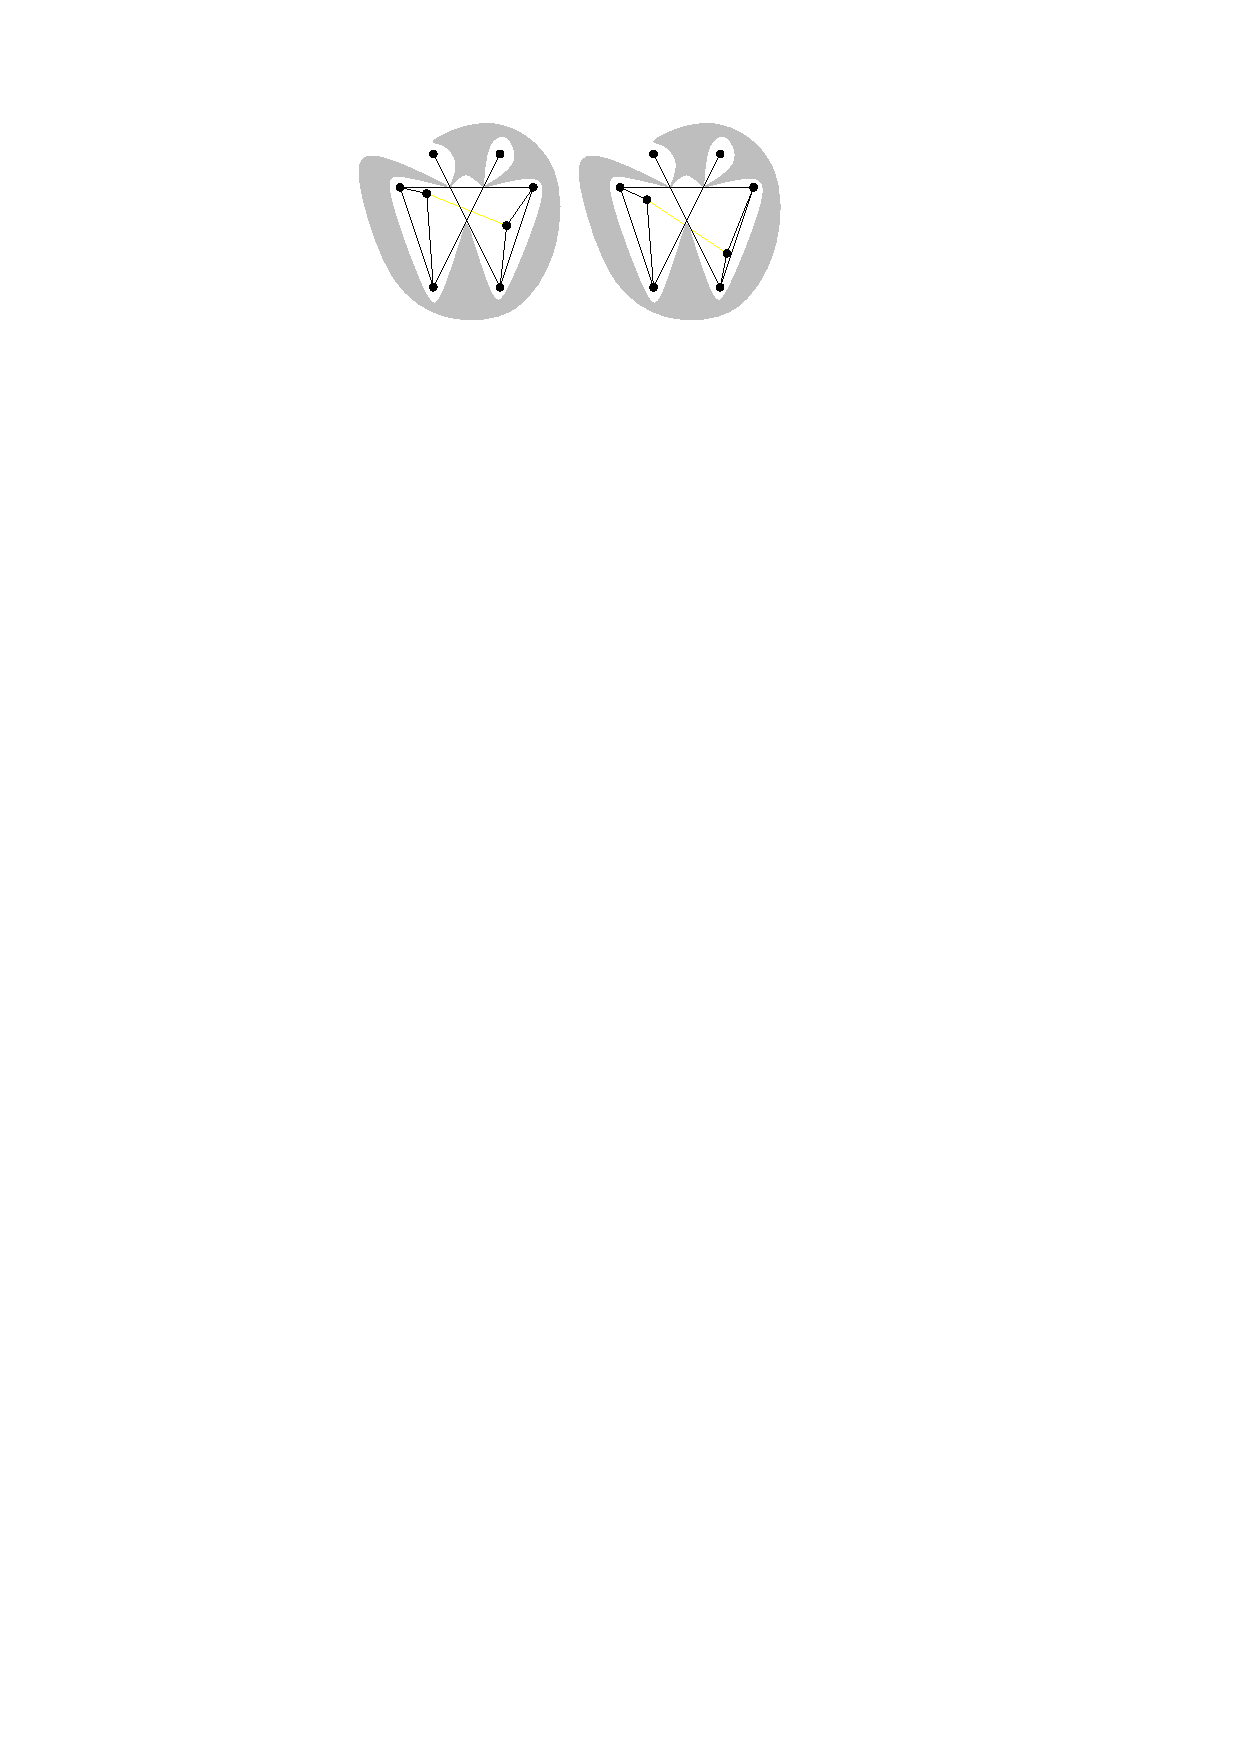
\includegraphics{order-type}
  \end{center}
  \caption{Order type and combinatorial type are insufficient to determine 
      the number of obstacles needed in an obstacle representation. The yellow
      segment represents a non-edge.}
  \figlabel{order-type-problem}
\end{figure}

The order type of the $\binom{n}{2}$ lines determined by the pairs of
vertices in the drawing \emph{is} sufficient to answer questions about
obstacle representations.  However, we are unaware of any sufficiently
strong upper bounds on the number of distinct order types of the
$\binom{n}{2}$ lines determined by $n$ points.

\subsection{Super-Order Types}

We now define an equivalence relation on point sets that is
strong enough for our purposes.  Consider a sextuple $T=\langle
a_1,a_2,b_1,b_2,c_1,c_2\rangle$ of points such that
\begin{enumerate}
  \item  $a_1\neq a_2$, $b_1\neq b_2$, $c_1\neq c_2$, 
  \item  $\{a_1,a_2\}\neq \{b_1,b_2\}$, 
$\{b_1,b_2\}\neq \{c_1,c_2\}$, $\{c_1,c_2\}\neq \{a_1,a_2\}$, and 
  \item $\{a_1,a_2\}\cap\{b_1,b_2\}\cap\{c_1,c_2\}=\emptyset$.
\end{enumerate}
We call a sextuple $T$ with this property an \emph{admissible} sextuple.
Let $A$ denote the directed line through $a_1$ and $a_2$ that is directed
from $a_1$ towards $a_2$. Define $B$ and $C$ similarly, but with respect
to $b_1,b_2$ and $c_1,c_2$, respectively.  We say that the sextuple,
$T$, is \emph{degenerate} if
\begin{enumerate}
  \item any of $A$, $B$, or $C$ is vertical;
  \item $A$ is parallel to $B$ or to $C$; or
  \item $A$, $B$, and $C$ contain a common point.
\end{enumerate}
\note{In your example, $A$, $B$, and $C$, share a common point, so they
are degenerate, so their type is 0.}
We define the \emph{type}, $\sigma(T)$, of $T$ as
\[
    \sigma(T) = \left\{\begin{array}{rl}
      -1 & \text{if $A\cap B$ comes before $A\cap C$ on $A$.} \\
      0 & \text{if $T$ is degenerate} \\
      +1 & \text{otherwise ($A\cap B$ comes after $A\cap C$ on $A$).} 
    \end{array}\right.
\]
(See \figref{super-order}.)  Let $\langle\langle
i_{1,\ell},i_{2,\ell},j_{1,\ell},j_{2,\ell},k_{1,\ell},k_{2,\ell}\rangle:
\ell \in \{1,\ldots,r\}\rangle$ be any sequence that lists the
admissible sextuples of the index set $\{1,\ldots,n\}$.  Note that $r<
\binom{n}{2}^3$.  The \emph{super-order type} of a sequence $P=\langle
x_1,\ldots,x_n\rangle$ of $n$ distinct points is the sequence
\[
   \sigma(P) = \left\langle \sigma\left(\left\langle x_{i_{1,\ell}},x_{i_{2,\ell}},
       x_{j_{1,\ell}},x_{j_{2,\ell}},
       x_{k_{1,\ell}},x_{k_{2,\ell}}\right\rangle\right) : \ell\in\left\{1,\ldots,r\right\} \right\rangle \enspace .
\]
Finally, we say that super-order type is \emph{simple} if it contains
no zeros and a sequence of points is \emph{simple} if its super-order
type is simple.  The following lemma shows that super-order types are
sufficient for answering questions about obstacle representations.

\begin{figure}[htbp]
  \begin{center}
    \begin{tabular}{cc}
       \includegraphics{super-order-1} &
       \includegraphics{super-order-2} \\ 
       -1 & 1 \\
    \end{tabular}\\[4ex]
    \begin{tabular}{ccc}
       \includegraphics{super-order-3} &
       \includegraphics{super-order-4} &
       \includegraphics{super-order-5} \\
       0 & 0 & 0
    \end{tabular}
  \end{center}
  \caption{The three cases of three lines defined by 6 points that can
      occur in the super-order type.}
  \figlabel{super-order}
\end{figure}

\begin{lem}\lemlabel{order-type}
  Let $G$ be a graph with vertex set $V=\{1,\ldots,n\}$ and let
  $\varphi_1\from V\to\R^2$ and $\varphi_2\from V\to\R^2$ be two drawings
  of $G$ such that $\langle\varphi_1(1),\ldots,\varphi_1(n)\rangle$
  and $\langle\varphi_2(1),\ldots,\varphi_2(n)\rangle$ have the same
  super-order type.  Then, if $G$ has an $h$-obstacle representation
  $(\varphi_1,S_1)$ then it also has an $h$-obstacle representation
  $(\varphi_2,S_2)$.
\end{lem}

\begin{proof}
  Consider the two plane graphs $G_1$ and $G_2$ obtained by
  adding a vertex where any two edges cross in the drawing
  $\varphi_1$, respectively, $\varphi_2$.  The fact that
  $\langle\varphi_1(1),\ldots,\varphi_1(n)\rangle$ and
  $\langle\varphi_2(1),\ldots,\varphi_2(n)\rangle$ have the same
  super-order type implies that $G_1$ and $G_2$ are two combinatorially
  equivalent drawings of the same planar graph.\note{This claim is the biggest hand-wave of the paper.}  Without loss of
  generality, we can assume that each obstacle $X_1\in S_1$ is an open
  polygon whose boundary is the face, $f_1$, of $G_1$ that contains $X_1$.
  For each such obstacle, we create an obstacle, $X_2\in S_2$, whose boundary
  is the face $f_2$ of $G_2$ that corresponds to $f_1$.  

  All that remains is to verify that an edge $uw$ is in $G_2$ if and
  only if the segment with endpoints $\varphi_2(u)$ and $\varphi_2(w)$
  does not intersect any obstacle in $S_2$.  By construction, no edge
  of the drawing $\varphi_2$ of $G$ intersects any obstacle in $S_2$.
  Furthermore, because $P_1$ and $P_2$ have the same super-order type,
  for every non-edge $uw$ of $G$, the segment $\varphi_2(u)\varphi_2(w)$
  intersects some obstacle in $S_2$.\note{Handwaving indeed, but justification is given in the next sentence.} (Indeed, $\varphi_2(u)\varphi_2(w)$
  intersects the obstacles of $S_2$ corresponding to those in $S_1$
  intersected by $\varphi_1(u)\varphi_1(w)$.)  That is, $(\varphi_2,S_2)$
  is an obstacle representation of $G$ using $h=|S_1|$ obstacles,
  as required.
\end{proof}

The next lemma shows that we can restrict our attention to drawings
onto simple point sets.

\begin{lem}\lemlabel{simple}
  If a graph $G$ with vertex set $V=\{1,\ldots,n\}$ has an
  $h$-obstacle representation $(\varphi, S)$, then $G$ has an
  $h$-obstacle representation $(\varphi',S')$ in which $\langle
  \varphi(1),\ldots,\varphi(n)\rangle$ is a simple point sequence.
\end{lem}

\begin{proof}
  We first note that, by rotation, we can assume that no two points in
  the image of $\varphi$ have the same x-coordinate.  Therefore, any
  degenerate sextuple in the image of $\varphi$ is not the result of
  a vertical line through two points in the sextuple.  Therefore, each
  degenerate sextuple is the result of two distinct parallel lines or of
  three lines passing through a common point.

  By growing the obstacles in $S$ into maximal open sets and then
  shrinking them slightly, we may assume that each obstacle in $S$ is
  an open set that is at some positive distance $\epsilon >0$ from each
  line segment $\varphi(u)\varphi(w)$ joining the two endpoints of each
  edge $uw$ in $G$.  Call this new set of obstacles $S'$.  We say that
  two points $a$ and $b$ are \emph{visible} if the open line segment
  with endpoints $a$ and $b$ does not intersect any obstacle in $S'$,
  otherwise we say that $a$ and $b$ are \emph{invisible}.

  We claim that, if the image of $\varphi$ is a non-simple point set,
  then some point $a_1=\varphi(u)$ is involved in a degenerate sextuple
  $T=\langle a_1,a_2,b_1,b_2,c_1,c_2\rangle$ that defines three lines $A$
  (containing $a_1$ and $a_2$), $B$ (containing $b_1$ and $b_2$), and
  $C$ (containing $c_1$ and $c_2$) such that (1)~$A$ is parallel to $B$;
  (2)~$A$ is parallel to $C$; or (3)~$A$, $B$, and $C$ are \emph{distinct}
  lines that contain a common point. In particular the case in which
  $B=C\neq A$ is ruled out. Refer to \figref{stupid-case} for what follows.
  To see why this claim is true, note that if we
  stumble upon the case in which $B=C\neq A$ then $b_1$, $b_2$, $c_1$, and
  $c_2$ are all collinear.  But then the admissible sextuple $T'=\langle
  b_1,b_2,c_1,c_2,a_1,a_2\rangle$ is also degenerate.  In this case, we
  can proceed by using the sextuple $T'$ which defines three lines $A'$
  (containing $b_1$ and $b_2$), $B'$ (containing $c_1$ and $c_2$), and
  $C'$ (containing $a_1$ and $a_2$) and in which $A'$ is parallel to $B'$.
  \begin{figure}
    \begin{center}
       \includegraphics{stupid-case}
    \end{center}
    \caption{A case we sidestep in the proof of \lemref{simple}.}
    \figlabel{stupid-case}
  \end{figure}

  Therefore, the degenerate sextuple $T$ defines one of the three cases
  in the bottom half of \figref{super-order}.  We claim that there
  exists a sufficiently small perturbation of $a_1$ that moves it to a
  new location $a_1'$ that simultaneously
  \begin{enumerate}
    \item[P1.] eliminates all the degenerate sextuples that include $a_1$;
    \item[P2.] does not change the type of any non-degenerate sextuple;
    \item[P3.] does not result in any point $b=\varphi(w)$ that is visible to $a_1$
      being invisible to $a_1'$; and
    \item[P4.] does not result in any point $b=\varphi(w)$ that is invisible to $a_1$
      being visible to $a_1'$.
  \end{enumerate}
  Note that the first two properties ensure that, by moving $a_1$ to $a_1'$,
  the number of degenerate sextuples decreases.  The last three properties
  ensure that the resulting drawing along with the obstacle set $S'$
  is an obstacle representation of $G$. We can easily verify that such
  a point $a_1'$ exists because:
  \begin{enumerate}
    \item[P1.] For each degenerate sextuple that includes $a_1$ there are only
    a constant number of directions $(a-a')/\|a-a'\|$ that preserve the
    degeneracy of that sextuple.  In particular, any direction not parallel
    to $A$, $B$, or $C$ works.
    \item[P2.] Changing the type of a non-denerate sextuple involving $a_1$
    requires moving $a_1$ by some distance $\delta >0$;  we can ensure
    that our perturbation moves $a_1$ by less than $\delta$.  
    \item[P3.] All obstacles are at distance $\epsilon >0$ from the
    edges of the drawing.  We can ensure that the perturbation moves
    $a_1$ by less than $\epsilon$. This ensures that any vertex visible to
    $a_1$ is also visible to $a_1'$.
    \item[P4.] All obstacles are open sets, so every non-edge intersects
    the interior of one or more obstacles.  In particular, there exists
    some $\delta >0$ such that, for each non-edge $uw$ there is a ball of
    radius $\delta$ whose center is on the segment $\varphi(u)\varphi(w)$
    and that is contained in some obstacle.  By moving $a_1$ by a
    distance of less than $\delta$, each such non-edge continues to
    intersect an obstacle.  That is, any vertex not visible to $a_1$
    is also not visible to $a_1'$.
  \end{enumerate}
  By properties P3 and P4, the preceding perturbation step results in
  a new mapping $\varphi_0$ such that $(\varphi_0,S')$ is an obstacle
  representation of $G$.  This perturbation also eliminates at least
  one degenerate sextuple (by property P1) and does not introduce any
  new degenerate sextuples (by property P2) so it decreases the total
  number of degenerate sextuples.  This step can therefore be repeated
  until no degenerate sextuples remain to obtain the desired $h$-obstacle
  representation $(\varphi',S')$.
\end{proof}

What remains is to show that $N$, the number of super-order types
corresponding to point sets of size $n$ is not too big.  Luckily,
the methods used by Goodman and Pollack \cite{goodman.pollack:upper}
to upper bound the numbers of order types and combinatorial types
generalize readily to super-order types.  The proof of the following
result is given in \appref{order-type}.

\begin{lem}\lemlabel{order-type-count}
  The number of sequences in $\{{-1},{+1}\}^{r}$ that are the super-order
  type of some simple point sequence of length $n$ is $e^{O(n\log n)}$.
\end{lem}

\subsection{Proof of \thmref{main}}

For completeness, we now spell out the proof of \thmref{main}.

\begin{proof}[Proof of \thmref{main}]
  Let $G=(V,E)$ be an Erd\H{o}s-R\'enyi random graph with $n$ vertices
  with vertex set $V=\{1,\ldots,n\}$.
  We say that the point sequence $\langle \varphi(1),\ldots,\varphi(n)\rangle$
  defined by an
  obstacle representation $(\varphi, S)$ \emph{supports} the obstacle
  representation.  Fix some simple super-order type on $n$ points.
  By \lemref{order-type}, all point sets with this super-order type
  support an obstacle representation of $G$ with $o(n/(\log\log n)^2)$
  obstacles or none of them do.  By \lemref{fixed}, the probability that
  all of them do is at most $p\le e^{-cn\log n}$ for every constant $c>0$.
  By the union bound and \lemref{order-type-count} the probability
  that there is any simple super-order type---and therefore any simple
  point set---that supports an obstacle representation of $G$ with
  $o(n/(\log\log n)^2)$ obstacles is
  \[
     \hat p = p\cdot e^{O(n\log n)} = e^{-cn\log n}\cdot e^{O(n\log n)} < 1
  \]
  for a sufficiently large constant $c$.  Therefore, with probability
  $1-\hat p > 0$, there is no simple point set that supports an obstacle
  representation of $G$ using $o(n/(\log\log n)^2)$ obstacles. We deduce
  that there exists some some graph, $G'$, with this property.  Finally,
  \lemref{simple} implies that we can ignore the restriction to simple
  point sets and deduce that $\obs(G')\in \Omega(n/(\log\log n)^2)$.
\end{proof}


\section{Remarks}

Our proof of \thmref{main} relates the problem of counting the number
of $n$-vertex graphs with obstacle number at most $h$ to the problem of
determining the worst-case obstacle number of a graph with $n$ vertices.
Currently, we use Mukkamala \etal's \thmref{pach-gang}, which proves an
upper-bound of $e^{O(hn\log^2 n)}$ on the number of $n$ vertex graphs
with obstacle number at most $h$.  Interestingly, their argument is an
encoding argument, which shows that any such graph can be encoded as the
order type of a set of $O(hn\log n)$ points followed by a list of the
points in this set that make up the vertices of the (polygonal) obstacles.
Their argument needs only order types (as opposed to super-order types)
since the point set that they specify includes the vertices of the
obstacles.

Any improvement on the upper-bound for the counting problem will
immediately translate into an improved lower-bound on the worst-case
obstacle number.  Let $f(h,k)$ denote the number of $k$-vertex graphs
with obstacle number at most $h$ and let 
\[  
   \hat h(k) = \max\left\{h:f(h,k) \le 2^{n^2/4}\right\} \enspace . 
\]
(The quantity $\hat h(k)$ is chosen so that a random graph
on $k$ vertices has probability at most $2^{-\Omega(k^2)}$ of having obstacle
number less than $\hat h(k)$.)
Our proof technique shows that
there exist graphs with obstacle number at least $n\hat{h}(c\log n)/(c\log
n)$. (\thmref{pach-gang} shows that $\hat{h}(k)\in\Omega(k/(\log k)^2)$.)

We note that our technique gives an improved lower bound until someone is
able to prove that $\hat h(n)\in\Omega(n)$.  At this point, a simpler
argument (see \cite[Theorem~3]{mukkamala.pach.ea:graphs}) shows that
there exists graphs with obstacle number at least $\hat{h}(n)$.

We conjecture that improved upper-bounds on $f(h,n)$ that reduce the
dependence on $h$ are the way forward:
\begin{conj}\conjlabel{h}
  $f(h,n) \le 2^{g(n)\cdot o(h)}$, where $g(n)\in O(n\log^2 n)$.
\end{conj}
In support of this conjecture, we observe that an upper bound of the
form $f(1,n)\le 2^{g(n)}$ is sufficient to give the crude upper bound
$f(h,n)\le 2^{h\cdot g(n)}$ since any graph with an $h$-obstacle
representation is the common intersection of $h$ graphs that each
have a 1-obstacle representation.  That is, if $\obs(G)\le h$, then
there exists $E_1,\ldots,E_h$ such that $G=(V,\bigcap_{i=1}^h E_i)$
and $\obs(V,E_i)=1$ for all $i\in \{1,\ldots,h\}$.  This seems like a
very crude upper bound in which many graphs are counted multiple times.
\conjref{h} asserts that this argument overestimates the dependence on $h$.


\section*{Acknowledgement}

This work was initiated at the \emph{Workshop on Geometry and Graphs},
held at the Bellairs Research Institute, March 10-15, 2013.  We are
grateful to the other workshop participants for providing a stimulating
research environment.

\note{I checked the accents on Sari\"oz and P\'alv\"olgyi. They use \textbackslash" in their papers.}
\bibliographystyle{abbrv}
\bibliography{obstacle}


\appendix

\section{Proof of \lemref{order-type-count}}
\applabel{order-type}

\begin{proof}[Proof of \lemref{order-type-count}]
   For a point, $p$, let $\x(p)$ and $\y(p)$ denote the x- and
   y-coordinate, respectively, of $p$.  Consider what it means for a
   sextuple $T=(a_1,a_2,b_1,b_2,c_1,c_2)$, which defines three lines
   $A$, $B$, and $C$, to be degenerate.  This can occur, for example,
   if $A$ and $B$ are parallel.  The lines $A$ and $B$ are parallel if
   and only if
   \[
      \x(a_1-a_2)\cdot \y(b_1-b_2) - 
       \x(b_1-b_2)\cdot \y(a_1-a_2) = 0 \enspace .
   \]
   (This formula is a formalization of the less precise statement
   ``the slopes of $A$ and $B$ are the same.'')
   Observe that the preceding equation is a polynomial in
   $a_1,a_2,b_1,b_2$ of degree 2.

   Next, consider the case where $T$ is degenerate because $A$, $B$, and
   $C$ intersect in a common point or because one of $A$, $B$, or $C$
   is vertical.  This occurs if and only if the following determinant
   is undefined or equal to zero:
   \begin{equation}
   \left|\begin{array}{lll}
   \y(a_1)-\x(a_1)\left(\frac{\y(a_1-a_2)}{\x(a_1-a_2)}\right) & \frac{\y(a_1)-\y(a_2)}{\x(a_1)-\x(a_2)} & 1 \\
   \y(b_1)-\x(b_1)\left(\frac{\y(b_1-b_2)}{\x(b_1-b_2)}\right) & \frac{\y(b_1)-\y(b_2)}{\x(b_1)-\x(b_2)}  & 1 \\
   \y(c_1)-\x(c_1)\left(\frac{\y(c_1-c_2)}{\x(c_1-c_2)}\right) & \frac{\y(c_1)-\y(c_2)}{\x(c_1)-\x(c_2)}  & 1 \\
   \end{array}\right| \enspace .
   \eqlabel{determinant}
   \end{equation}
   (The values in this matrix are the $\y$-intercepts and slopes of the
   lines $A$, $B$, and $C$.)
   Multiplying the matrix in \eqref{determinant} by 
   \[
      \x(a_1-a_2)\cdot
      \x(b_1-b_2)\cdot
      \x(c_1-c_2)
   \]
   yields a polynomial of degree $6$ in the six variables
   $a_1,a_2,b_1,b_2,c_1,c_2$ that is equal to zero if and only if $A$,
   $B$, and $C$ contain a common point or one of $A$, $B$, or $C$
   is vertical. (Recall that $\det(cA)=c^r\cdot\det(A)$ when $A$ is a
   $r\times r$ matrix.)

   For the remainder of the proof, we proceed exactly as in
   Reference~\cite{goodman.pollack:upper}.  We can treat any sequence of $n$
   points in $\R^2$ as a single point in $\R^{2n}$.  Applying the
   preceding conditions for determining the degeneracy to each of
   the $O(n^6)$ admissible sextuples of points results in a set of
   $O(n^6)$ polynomials in $2n$ variables, each of constant degree.
   By multiplying these polynomials together, we obtain a single
   polynomial, $P^*$, in $2n$ variables and having degree $d\in O(n^6)$.
   If $X\subset\R^{2n}$ is the zero set of $P^*$, then $\R^{2n}\setminus
   X$ has at most $(2+d)^{2n}=e^{O(n\log n)}$ connected components
   \cite[Lemma~2]{goodman.pollack:upper}.\note{The \# components argument is usually called the Milnor-Thom bound, but it has a long history---see
the footnote on Page 4 here: \url{http://goo.gl/XtpVyR}.}

   Observe that $X$ corresponds exactly to the set of non-simple
   point sequences and observe that a sextuple of points cannot be moved
   continuously so that its type goes from $-1$ to $+1$, or vice versa,
   without its type becoming $0$ at some point during the movement.
   In particular, it is not possible to change the super-order type of
   a simple point sequence without going through a non-simple super-order type.
   Thus, within each component, $C$, of $\R^{2n}\setminus X$, the
   super-order type corresponding to every point in $C$ is the same.
   We conclude that the number of super-order types of simple point
   sequences is at most the number of components of $\R^{2n}\setminus X$,
   which is $e^{O(n\log n)}$, as required.
\end{proof}

\section*{Authors}

%\noindent
%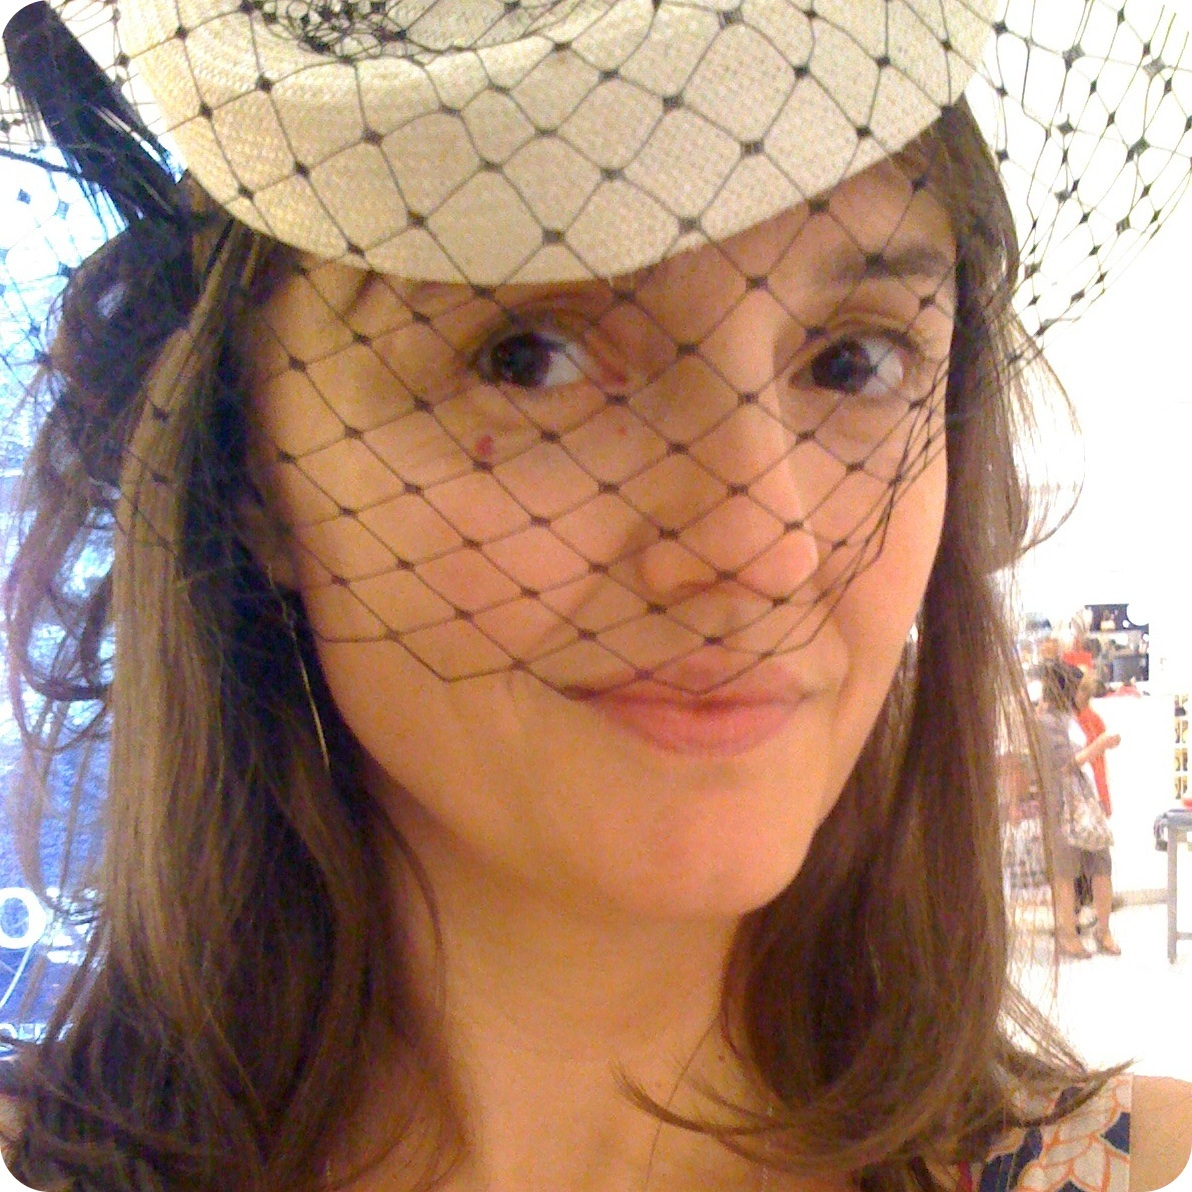
\includegraphics[width=.45\textwidth]{vida-b}% 
%\hspace{.1\textwidth}%
%
\includegraphics[width=.45\textwidth]{pat-b}%

\noindent\emph{Vida Dujmovi\'c.}
School of Mathematics and Statistics and Department of Systems and Computer Engineering, Carleton University
%, \texttt{vida@cs.mcgill.ca}

\noindent\emph{Pat Morin.}
School of Computer Scence, Carleton University
%, \texttt{\{morin,smid\}@scs.carleton.ca}




\end{document}



